\documentclass{article}

%Um mit Latex zu arbeiten braucht man zwei Dinge:
% https://miktex.org/download
% https://www.xm1math.net/texmaker/download.html

%Hilfreiche Links:
%Sonderzeichen in Latex einfügen: https://de.wikibooks.org/wiki/LaTeX-Kompendium:_Sonderzeichen

\usepackage{xcolor} %Hier wird ein Paket eingefügt, welches Text farbig machen kann
\usepackage{graphicx}
\usepackage{mathtools} %Das muss man noch installieren (man wird beim ersten Ausführen des Codes darauf hingewiesen und kann das dann direkt mit 'install' tun)

\begin{document} 

\title{Gaussian beam optics}
\author{Corinna Elena Wegner, Garen Gregorian}
\date{June 8, 2022}
\maketitle %hiermit wird das Deckblatt erst erstellt
\newpage
\tableofcontents
\newpage

\section{Einleitung} %dies ist eine Überschrift
\subsection{Dies ist eine Überschrift zweiten Ranges}
%Wenn ich \subsection* schreibe (mit *), kommt diese Überschrift nicht in die Gliederung

in diesem Versuch soll das Intensitätsprofil von Gaußschen Strahlen vermessen und die Auswirkungen von optischen Elementen untersucht werden\\
%Das muss noch auf Englisch übersetzt werden
%\\ macht einen Zeilenumbruch
%Formeln mit $Formeln$ einfügen
%Wichtigere Formeln mit \[ Formel \]

\textcolor{red}{Genereller Versuchsaufbau mit Skizze}\\
%Dinge die nicht Text sind sondern Dinge die noch rein müssen bzw. TO-DOs hab ich für uns zum Überblick rot gemacht 

\section{Measuring the power of the laser}

In the first part we measured the power of the laser itself. First, we put a photodiode with internal resistance 100k$\Omega$
after the first passive reflector and measured the voltage
\ $U=(1.2 \pm 0.1) V$ %So bindet man Formeln in Text ein
. Then we turned the laser off and measured again at the same position to eliminate the background light (the windows were covered by curtains). We measured 
\ $U_b = (1.2 \pm 0.1)mV$ 
using the 
10k$\Omega$
photodiode. 

\textcolor{red}{add answer, fehlerrechnung, make sure to say we incoroprated the fact that the diode resistances were different and add sktech of experimental set up, answer all questions page 11}

Though we used a voltmeter, but an Oscilloscope with a known measuring resistance $R_m$ can just as well be used. With the measured voltage $V_m$ one can conclude the photocurrent $I_p = V_m \cdot R_m$. To ensure an accurate measurement, we would want $R_m >>R_i$ since

\paragraph{}

$\frac{1}{R_{total}}= \frac{1}{R_m}+\frac{1}{R_i}$

\paragraph{}

and for sufficiently large $R_i$:
$\hspace{3}$
$\frac{1}{R_{total}} \approx \frac{1}{R_m} \rightarrow R_{total} = R_m$




\paragraph{Calculating the power from the voltage}

When the beam hits the diode, the multimeter detects a voltage $U$. For photodiodes, the relation between the power and light current ist given by 
\begin{equation} 
P = \frac{hfI}{e\eta}
\end{equation}
Here, $h = 6.62607015*10^{-34} Js$ is the planck constant, $e = 1.602176634*10^{-19} C$ the charge of an electron, $I$ is the current and $\eta = 0.75$ the quantum efficiency of the photodiode. We can replace the frequency $f$ in the formula by the corresponding wavelength $\lambda = 632.8 nm$ of the laser using $c= \lambda f$, with the vacuum speed of light  $c = 299792458 \frac{m}{s}$. Using ohm's law $ U= R \cdot I$ we eliminate the current $I$ and obtain 
\begin{equation}
P = \frac{hcU}{\lambda Re \eta}
\end{equation}


\textcolor{red}{Wie Formeln nummerieren? Quellenverzeichnis! https://de.wikipedia.org/wiki/Quantenausbeute}

The resistance $R$ can be read from the photodiode. In the experiment we used two diodes, mainly diode 1 with $R=10 k\Omega$. Diode 2 has $R= 100 k\Omega$. Thus by plugging the respective values in, we can calculate:
\paragraph{}

$P_{Laser} =  \frac{6.62607015*10^{-34}\cdot299792458\cdot1.2}{632.8\cdot10^{-9}\cdot1.602176634*10^{-19}\cdot0.75\cdot100000}=3.13*10^{-5} \vspace{2}$

$\Delta P_{Laser}= \pm \frac{6.62607015*10^{-34}\cdot299792458\cdot0.1}{632.8\cdot10^{-9}\cdot1.602176634*10^{-19}\cdot0.75\cdot10^{5}} =\pm 0.27*10^{-5} \vspace{2}$

$P_{Background} =  \frac{6.62607015*10^{-34}\cdot299792458\cdot1.2*10^{-3}}{632.8\cdot10^{-9}\cdot1.602176634*10^{-19}\cdot0.75\cdot10^{4}}=0.03*10^{-5} \vspace{2}$

$\Delta P_{Background} = \pm \frac{6.62607015*10^{-34}\cdot299792458\cdot0.1}{632.8\cdot10^{-9}\cdot1.602176634*10^{-19}\cdot0.75\cdot10^{5}} =\pm 0.27*10^{-7} \vspace{2}$


\paragraph{}

Thus by subtraction we can determine the power of the laser without any background influence as

\paragraph{}


$P^{'}_{Laser} = 3.13*10^{-5}- 0.03*10^{-5} =3.10*10^{-5} \pm 0.27*10^{-5}$

\paragraph{}
Since the background power is outside of the measurement error of
the laser power measurement, we cannot ignore the background power, however the difference is so low that one can safely expect results to not change much in a dimmed and normally lit room. A lit room, however, allows for more accurate measurements since observation of scales and thus of measurements becomes easier to the human eye and there are fewer risks of bumping into instruments or the table, thus reducing the chance of misallignments and accidentally influencing measurements.
\textcolor{red}{Fehlerquellen: Lichtstrahl hat Diode nicht perfekt fokussiert, verluste?}

\section{Coupling the optical fibre cables}

After determining the power of the laser we coupled the fibre optic cables into the coupler in the optical path. First, we coupled the multimode cable and adjusted the optical elements such that the conduction was optimized. By variating the angles a little we tried to see different modes on a piece of paper, put behind the cable. Unlike our expectations we could not identify them, instead the dot on the paper disappeared, because too few light was conducted through the cable. We could however see on the paper a dot with a small dark hole in it's center, just like the shape of a donut mode. It is also possible that the small hole was a dust crumb on the lens whatsoever. Unfortunately it was not possible to take a picture of the dot which shows more than a diffuse point, because the mobile phone cameras could not work with the light conditions.\\

Now we measured the voltage from the photodiode behind the cables. Therefor we focused the beam into the photodiode, using another lens. For the multimode cable we measured a maximum voltage of $U=209mV$, but the value fluctuated a lot (about 20mV just from touching the table). After coupling the single mode cable we measured $U=(106 \pm 5)mV$. This is less than for the multimode cable, which makes sense because there is only one mode lead through the single mode cable. With the resistance of the used photodiode, $R = 10k\Omega$, we can calculate the percentage of the power lead through the cable:


\paragraph{}
The corrected laser power translates to a corrected voltage value for the Laser of 
\paragraph{}

$U'_{Laser}= 1.19 \pm 0.11 V$

$\vspace{1}$

$U_{single-mode} =(106 \pm 5)mV  \hspace{1cm} U_{multi-mode} = (209\pm 20)mV$

$\vspace{1}$

$\eta_{single-mode} = \frac{106}{1.19*10^3} = 8.93\% \hspace{1cm} \eta_{single-mode} = \frac{209}{1.19*10^3} = 17.61\%$

$\vspace{1}$

$\Delta\eta_{sinlge-mode} = \pm8.93\%\cdot(\frac{5}{106}+ \frac{0.11}{1.19})= \pm 1.25\%$

$\vspace{1}$

$\Delta\eta_{single-mode} =\pm17.61\%\cdot(\frac{20}{209}+\frac{0.11}{1.19})= \pm 3.32\%$

$\vspace{1}$

$\xrightarrow[]{} \eta_{single-mode} = 8.93\pm 1.25\%\hspace{1cm}\Delta\eta_{sinlge-mode}=17.61\pm 3.32\%$

$\vspace{1}$

As expected, the multi mode cable has a higher efficiency since it allows for more modes to be transmitted. The measured efficiency was highly dependent on the sensitive alignment of the laser. This is especially true for the single mode photodiode since it has a smaller lens diameter. We can therefore expect that energy has been lost due to imperfect alignment and other various smaller inefficiencies, such as optical instruments heating up. The influence of dust particles on the lens of the photodiode is also noteworthy as a factor that further lowers efficiency. During the experiment it had a significant impact on the observed laser projection.
\textcolor{red}{Fehlerquellen:
-kabel Beschädigt: keine perfekte Leitung durch kabel, Fehler aus TV1}

\section{Measuring the beam profile}

In this experiment we measured the intensity of the laser light that is emitted by the fibre. We cut off some of the beam with a razor blade to see how much voltage is still measured by the photodiode. Thereby we obtained a profile of the beam cross section. After that we put a lens ($f=100mm$) behind the fibre end so that the beam was focused at the focal point. We measured the profile of the beam at different positions between the two lenses (the second lens ($f=50mm$) focuses the beam into the photodiode). Near the focal point of the first lens, where the waist of the gaussian beam lies, we measured three times. To eliminate influences from ambient light, we normalized the voltage signal with the other photodiode.\\

The total power the photodiode is detecting depends on the position of the razor blade $x$ and is given by:
\begin{equation}
P(x) = \int_x^\infty\mathrm{d}x' I_0 \mathrm{e}^{-\frac{2(x'-x_0)^2}{\omega^2}}.
\end{equation}

\textcolor{red}{Beantworten: Welches Brechungsindexprofil müßte eine Glasfaser aufweisen, damit die Faser eine ideale Gauß-Mode führt?}

\paragraph{Measuring the cross section profile without focusing the beam}

To calculate the beam radius $\omega (z)$ we fitted the data of our measurement a (see annex)
\textcolor{red}{Anhang hinzufügen} %and waist $\omega$ 
to the power integral. In order to do this we calculated the power from the voltage using eq. \\
\textcolor{red}{Formelnummerierung}

\includegraphics[width=\textwidth]{part a: cross section profile of collimated beam.png}

The first two measurements of the series with $Distance razor blade - fibre end = 8.3 cm$ seemed to fall out of line. When doing the fit, the curve (red dashed) also looked inappropiate. Presumably we measured these points too early, namely not at the point right before the power falls off (i.e. the maximum). Therefore we decided to leave them out of the fitting, which lead to a much better result (see figure ).
\textcolor{red}{which figure number?}
The resulting parameters from the fitting are: \\

For $Distance razor blade - fibre end = 11.0 cm$ the waist is negative, which is impossible and therefore we left this value out in the calculation of the average waist. Since this measurement series was taken at the furthest point from the beam origin, we assume that generally the influence of error sources are much higher than for measurements taken close to the beam origin.\\

\textcolor{red}{include parameters of csv datei a;Interpretation! Ziel war, $\omega$ zu bestimmen.;alle zahlenwerte;messungenauigkeiten;Fehlerquelle: streuendes licht; Am Ende Prüfen ob im Pythoncode die richtigen formeln benutzt wurden, outputs von pythoncode einfügen und diskutieren}

\paragraph{Measuring the cross section profile with lens ($f=100mm$)}

We measured the beam profile using the razor blade technique at seven distances from the lens. Three measurements were taken near the focal point because here we expected the waist $\omega_{0}$, i.e. the minimum of the beam radius $\omega (z)$. They are related by the equation:
\begin{equation}
\omega (z) = \omega_{0}\sqrt{1+\frac{z^2}{z_{R}^2}},
\end{equation}

The razorblade positions z from which we measured the beam profile are $-(7.0\pm 0.2)cm, -(4.0\pm 0.2)cm, -(1.0\pm 0.2)cm, (0.0\pm 0.2)cm, (1.0\pm 0.2)cm, (4.3\pm 0.2) cm$ and $(7.0\pm 0.2)cm$, where $z=0$ is the focal point. For better clearness we plotted the data near focal point in an extra plot. The plots show the calculated powers (eq.) from the measuring data along with the corresponding Fit to the gaussian integral (eq.). From the fit we obtained $I_{0}$ and $\omega(z)$.: \\ 

\textcolor{red}{formelnummerierung und Daten aus pythoncode einfügen}
The value $\omega(7cm) = ... $ is negative and therefore illogical. Therefore we left it out from further calculations. Again this measurement series was taken from the furthest point from the fibre end, so we assume generally higher influence from error sources of any kind\\

We fitted the values $\omega(z)$ to eq. $\omega (z) = \omega_{0}\sqrt{1+\frac{z^2}{z_{R}^2}}$ and eventually obtained the waist $\omega_{0}$ and rayleigh length $z_{R}$ as fit parameters: 
\textcolor{red}{include results} 

where 
\begin{equation}
z_{R} = \frac{\pi\omega_{0}^2 n}{\lambda} 
\end{equation}
 is the rayleigh length, at which the beam radius is $\sqrt{2}\omega_{0}$. In our case, $n=1$ is the refraction index of the medium (air) and the wavelength of the laser is $\lambda = 632.8 nm$.\\

Again, we fitted the measurement series for each razor-lens-distance $z$ to the power integral and obtained the local $\omega(z)$. Then we fitted these together with the corresponding $z$ to eq. []
\textcolor{red}{nummerierung}.
From that we obtained the waist 
\textcolor{red}{$\omega_{0} = ...$ }
The resulting rayleigh length is 
\textcolor{red}{zR ...}

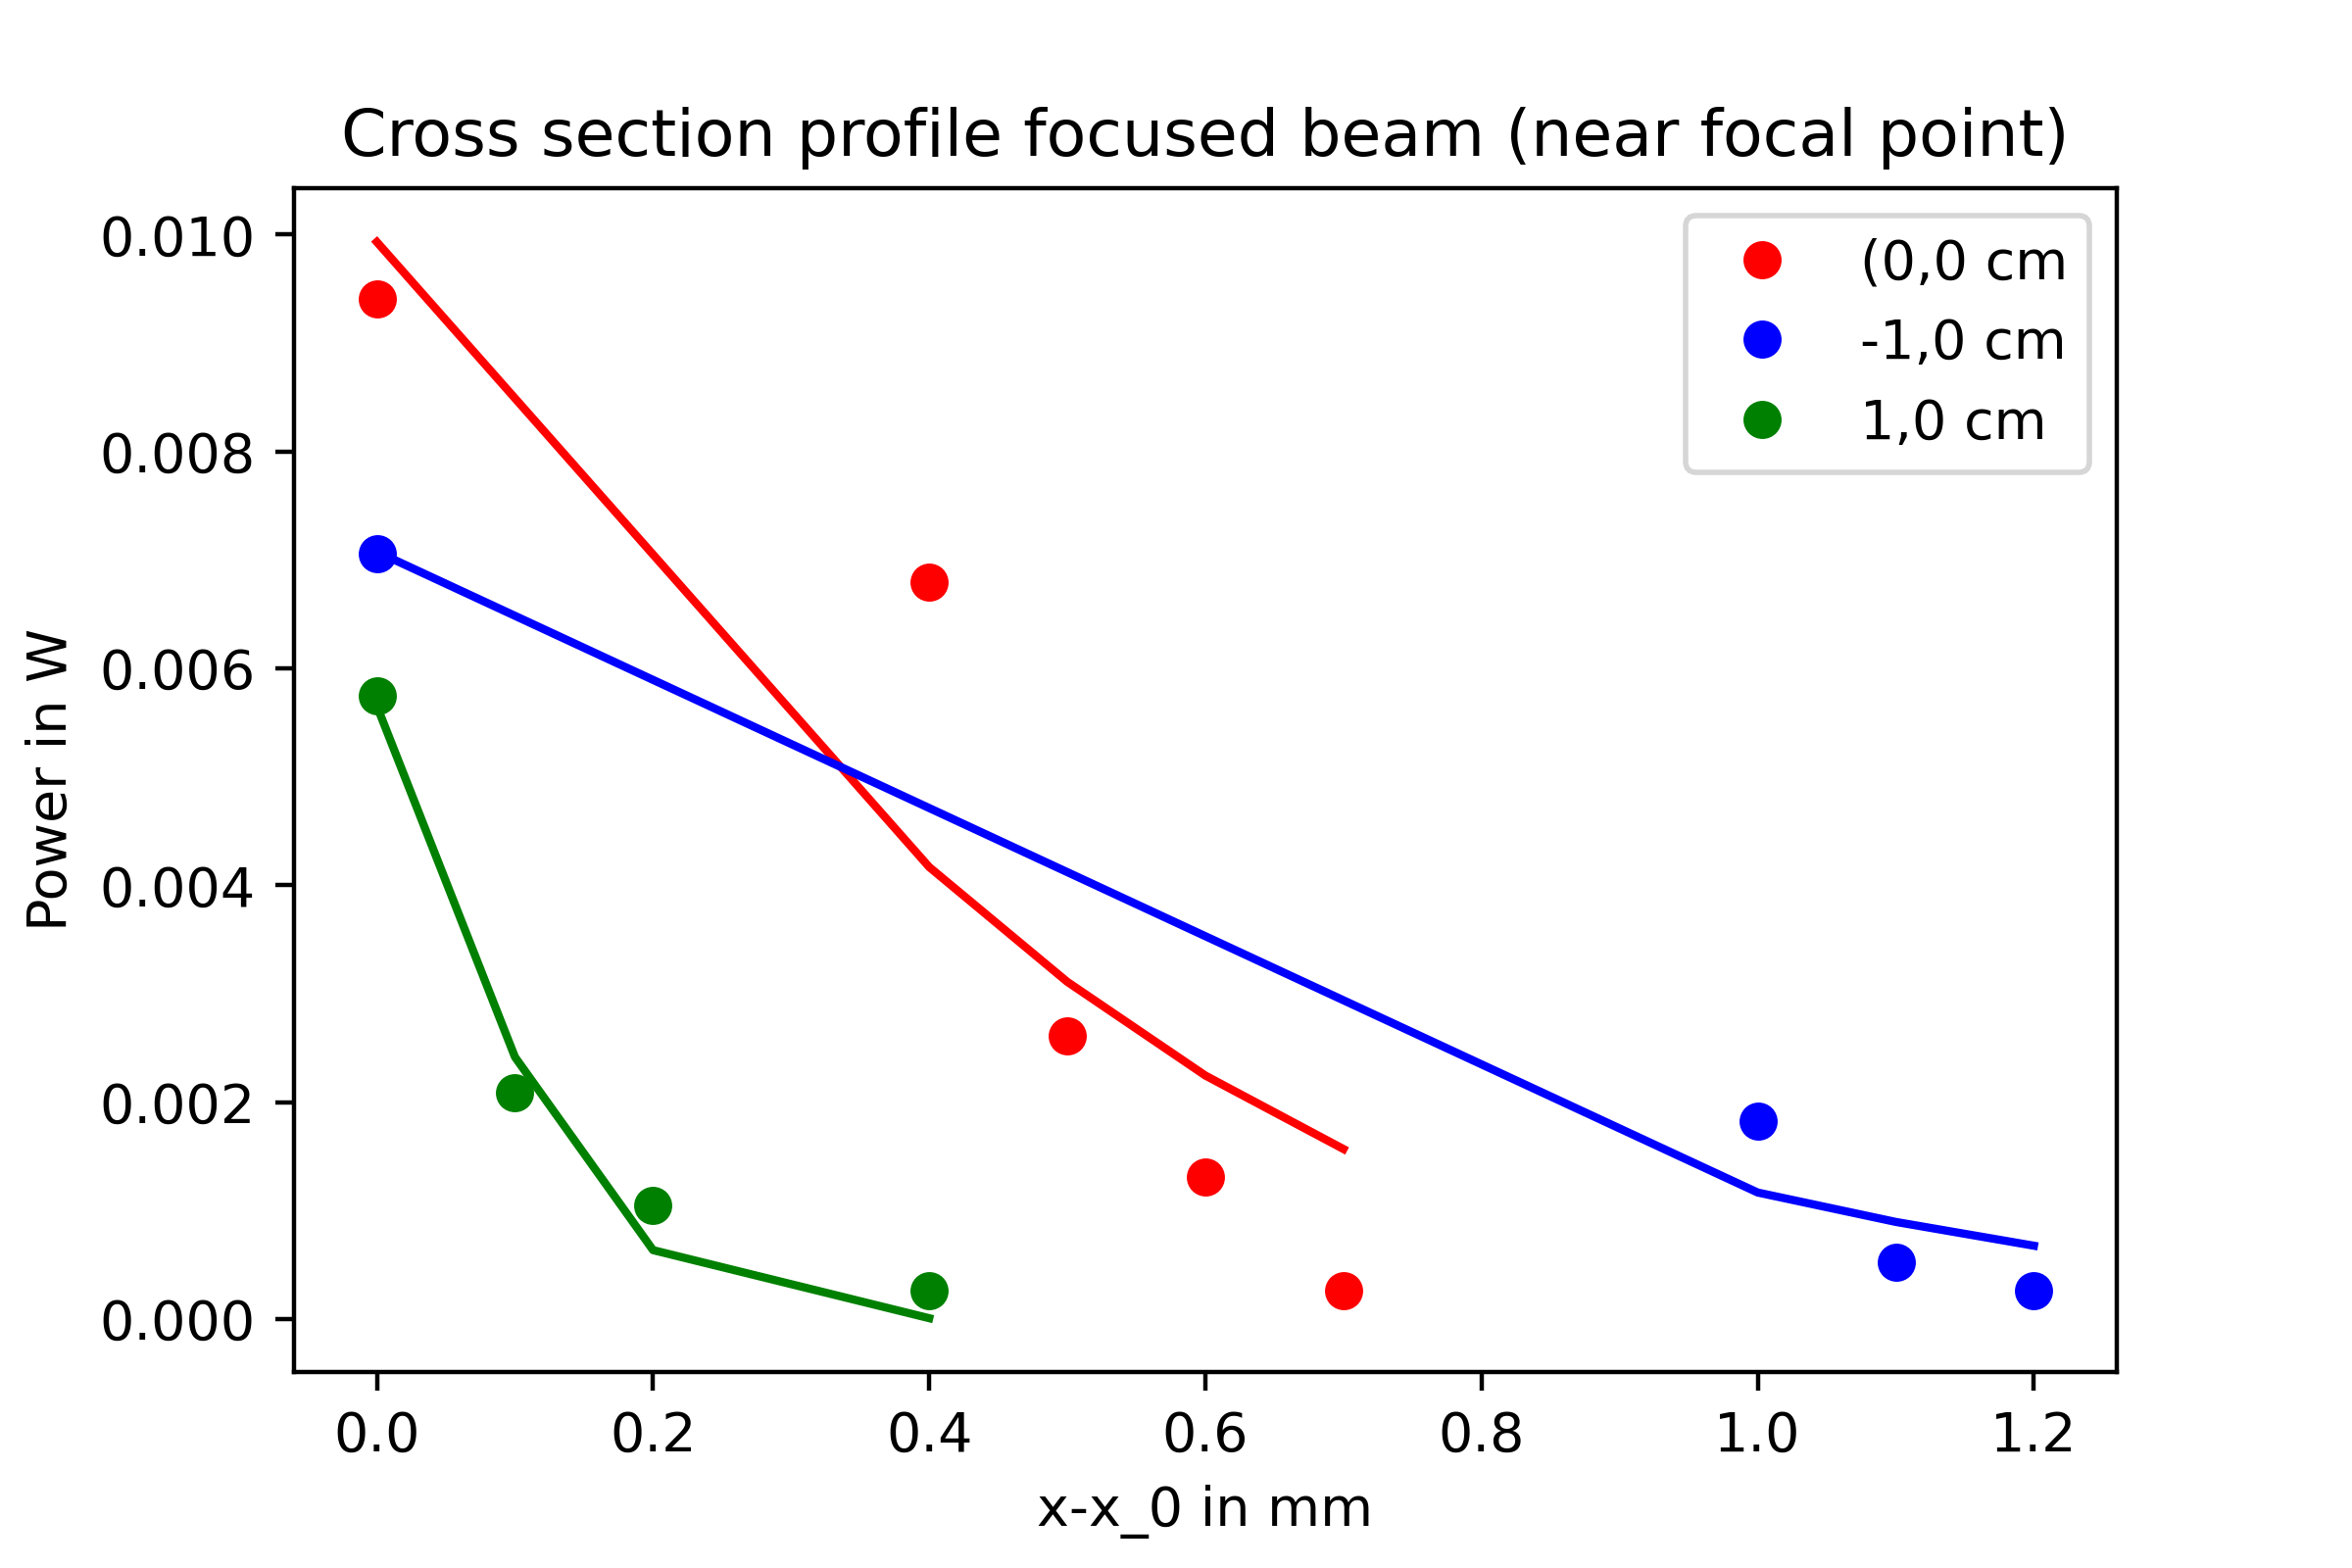
\includegraphics[width=\textwidth]{Cross section profile focused beam (near focal point).png} %muss noch richtig skalieren
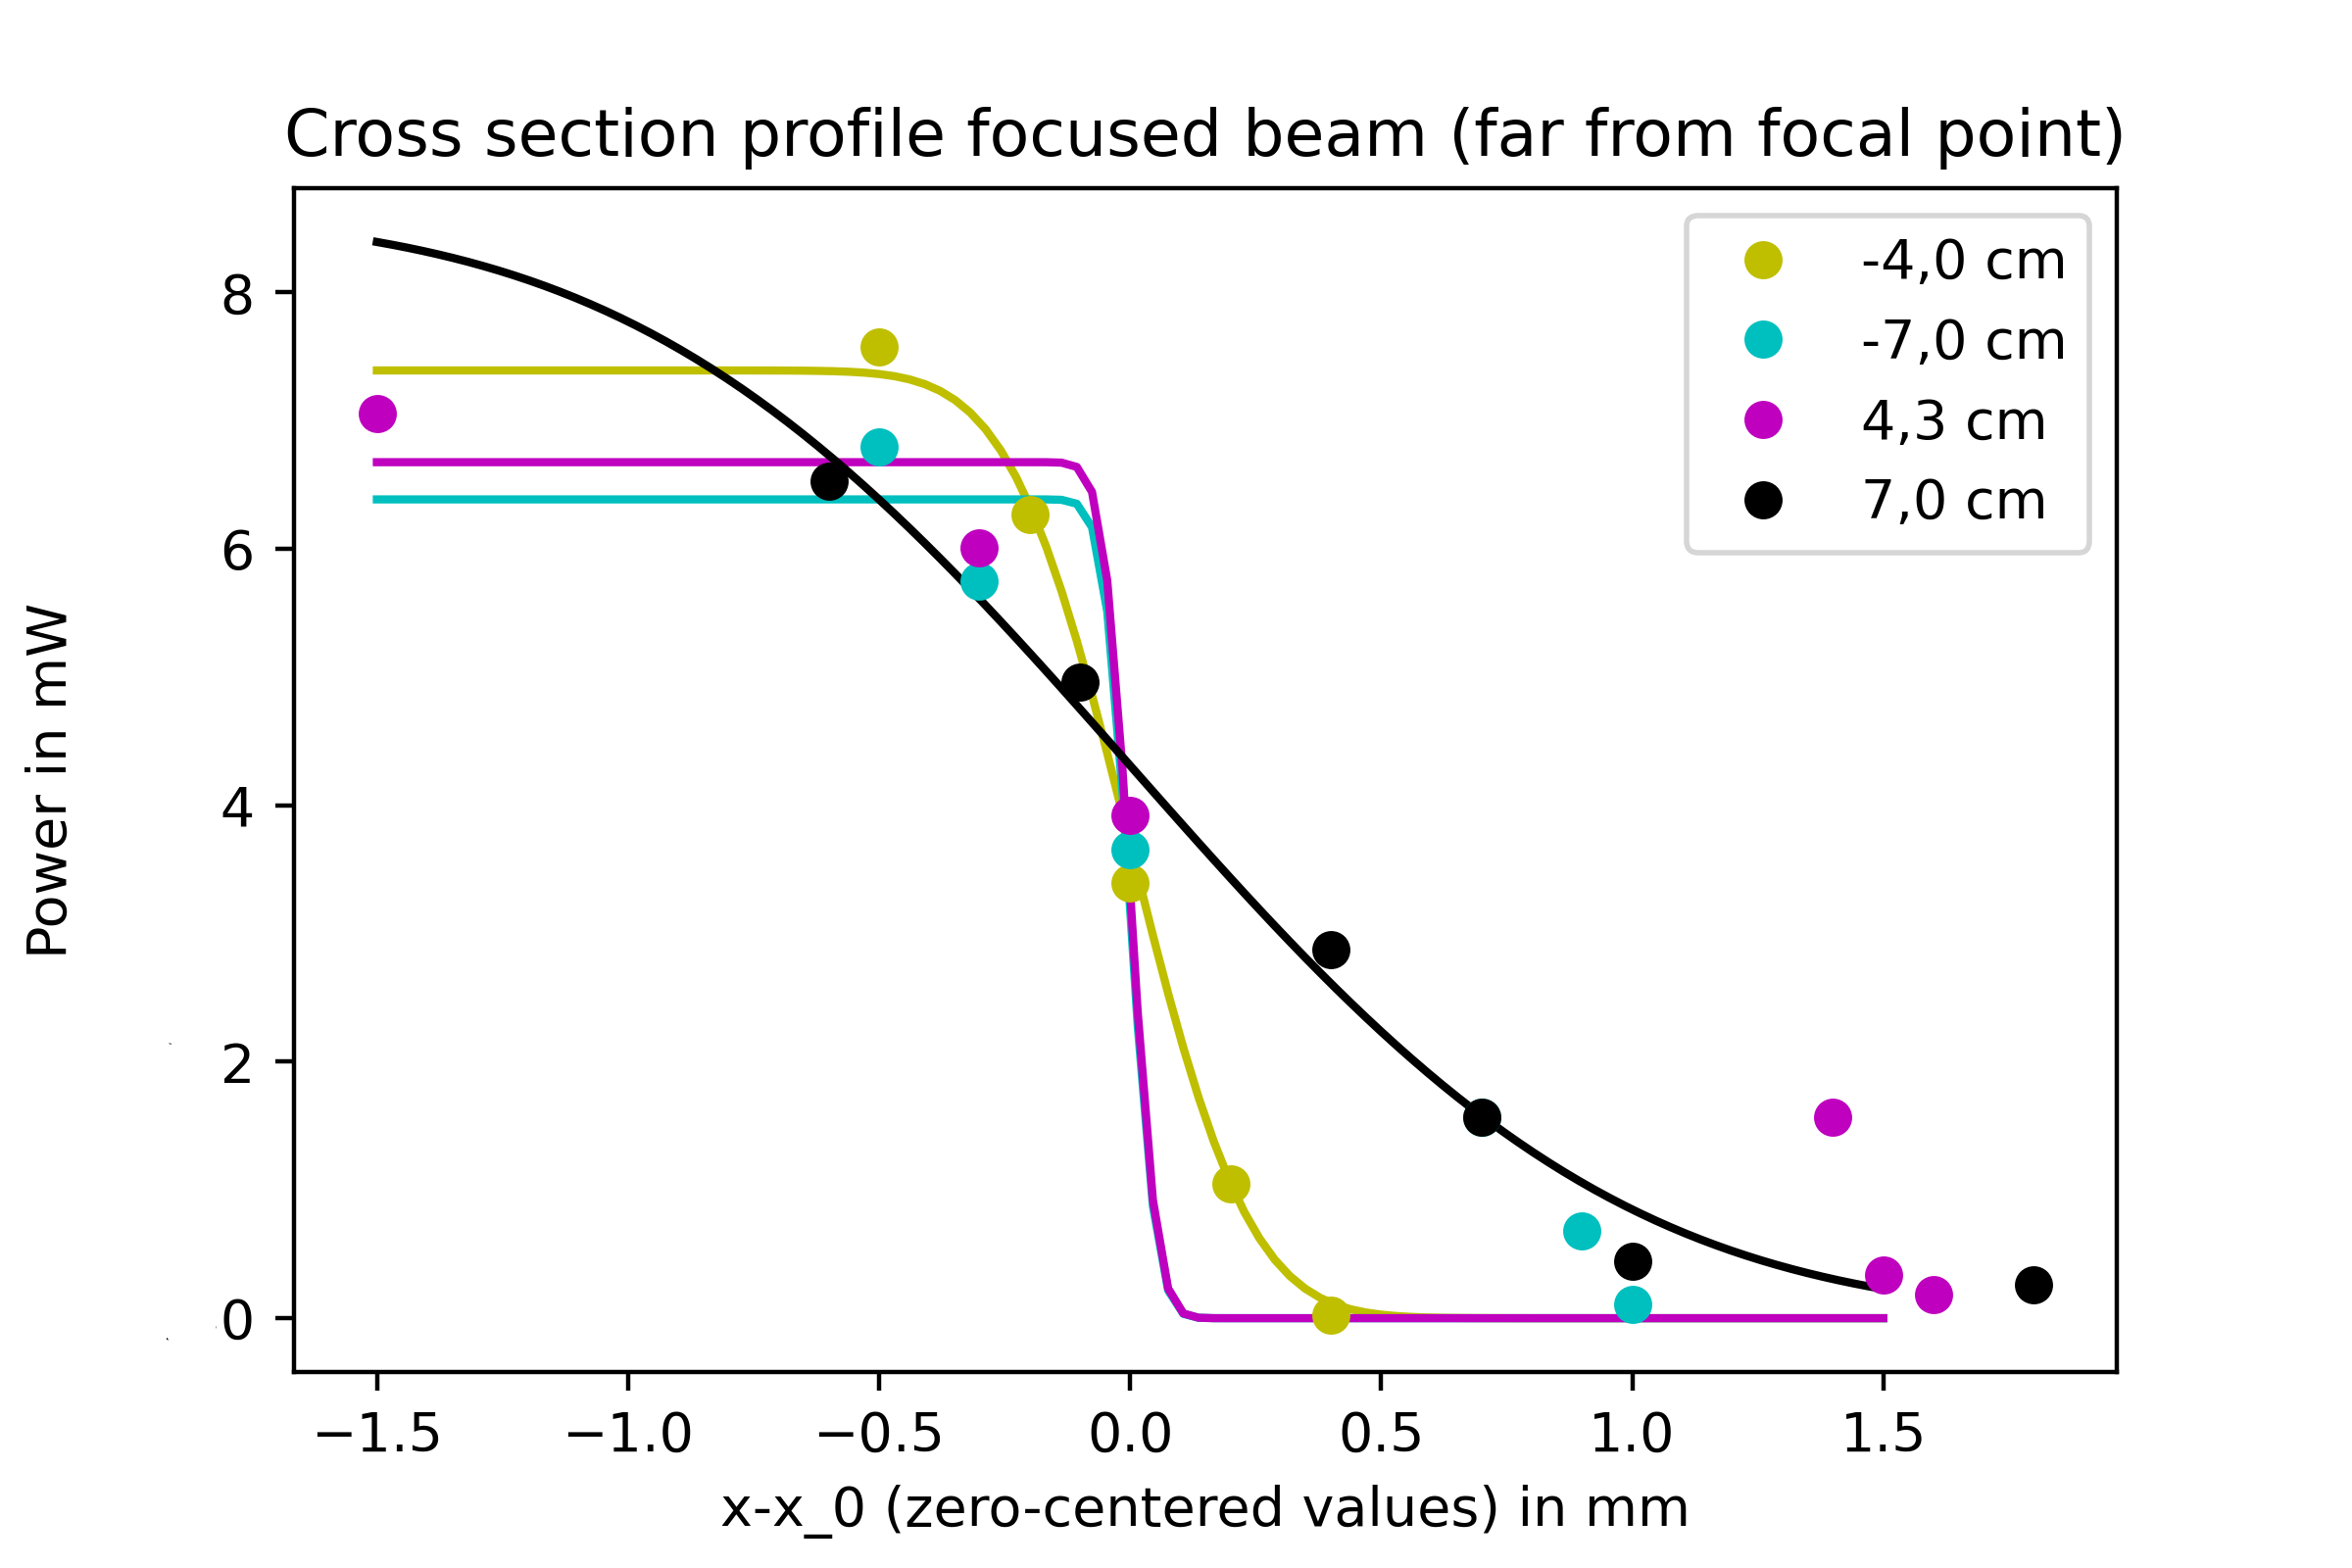
\includegraphics[width=\textwidth]{Cross section profile focused beam (far from focal point).png}
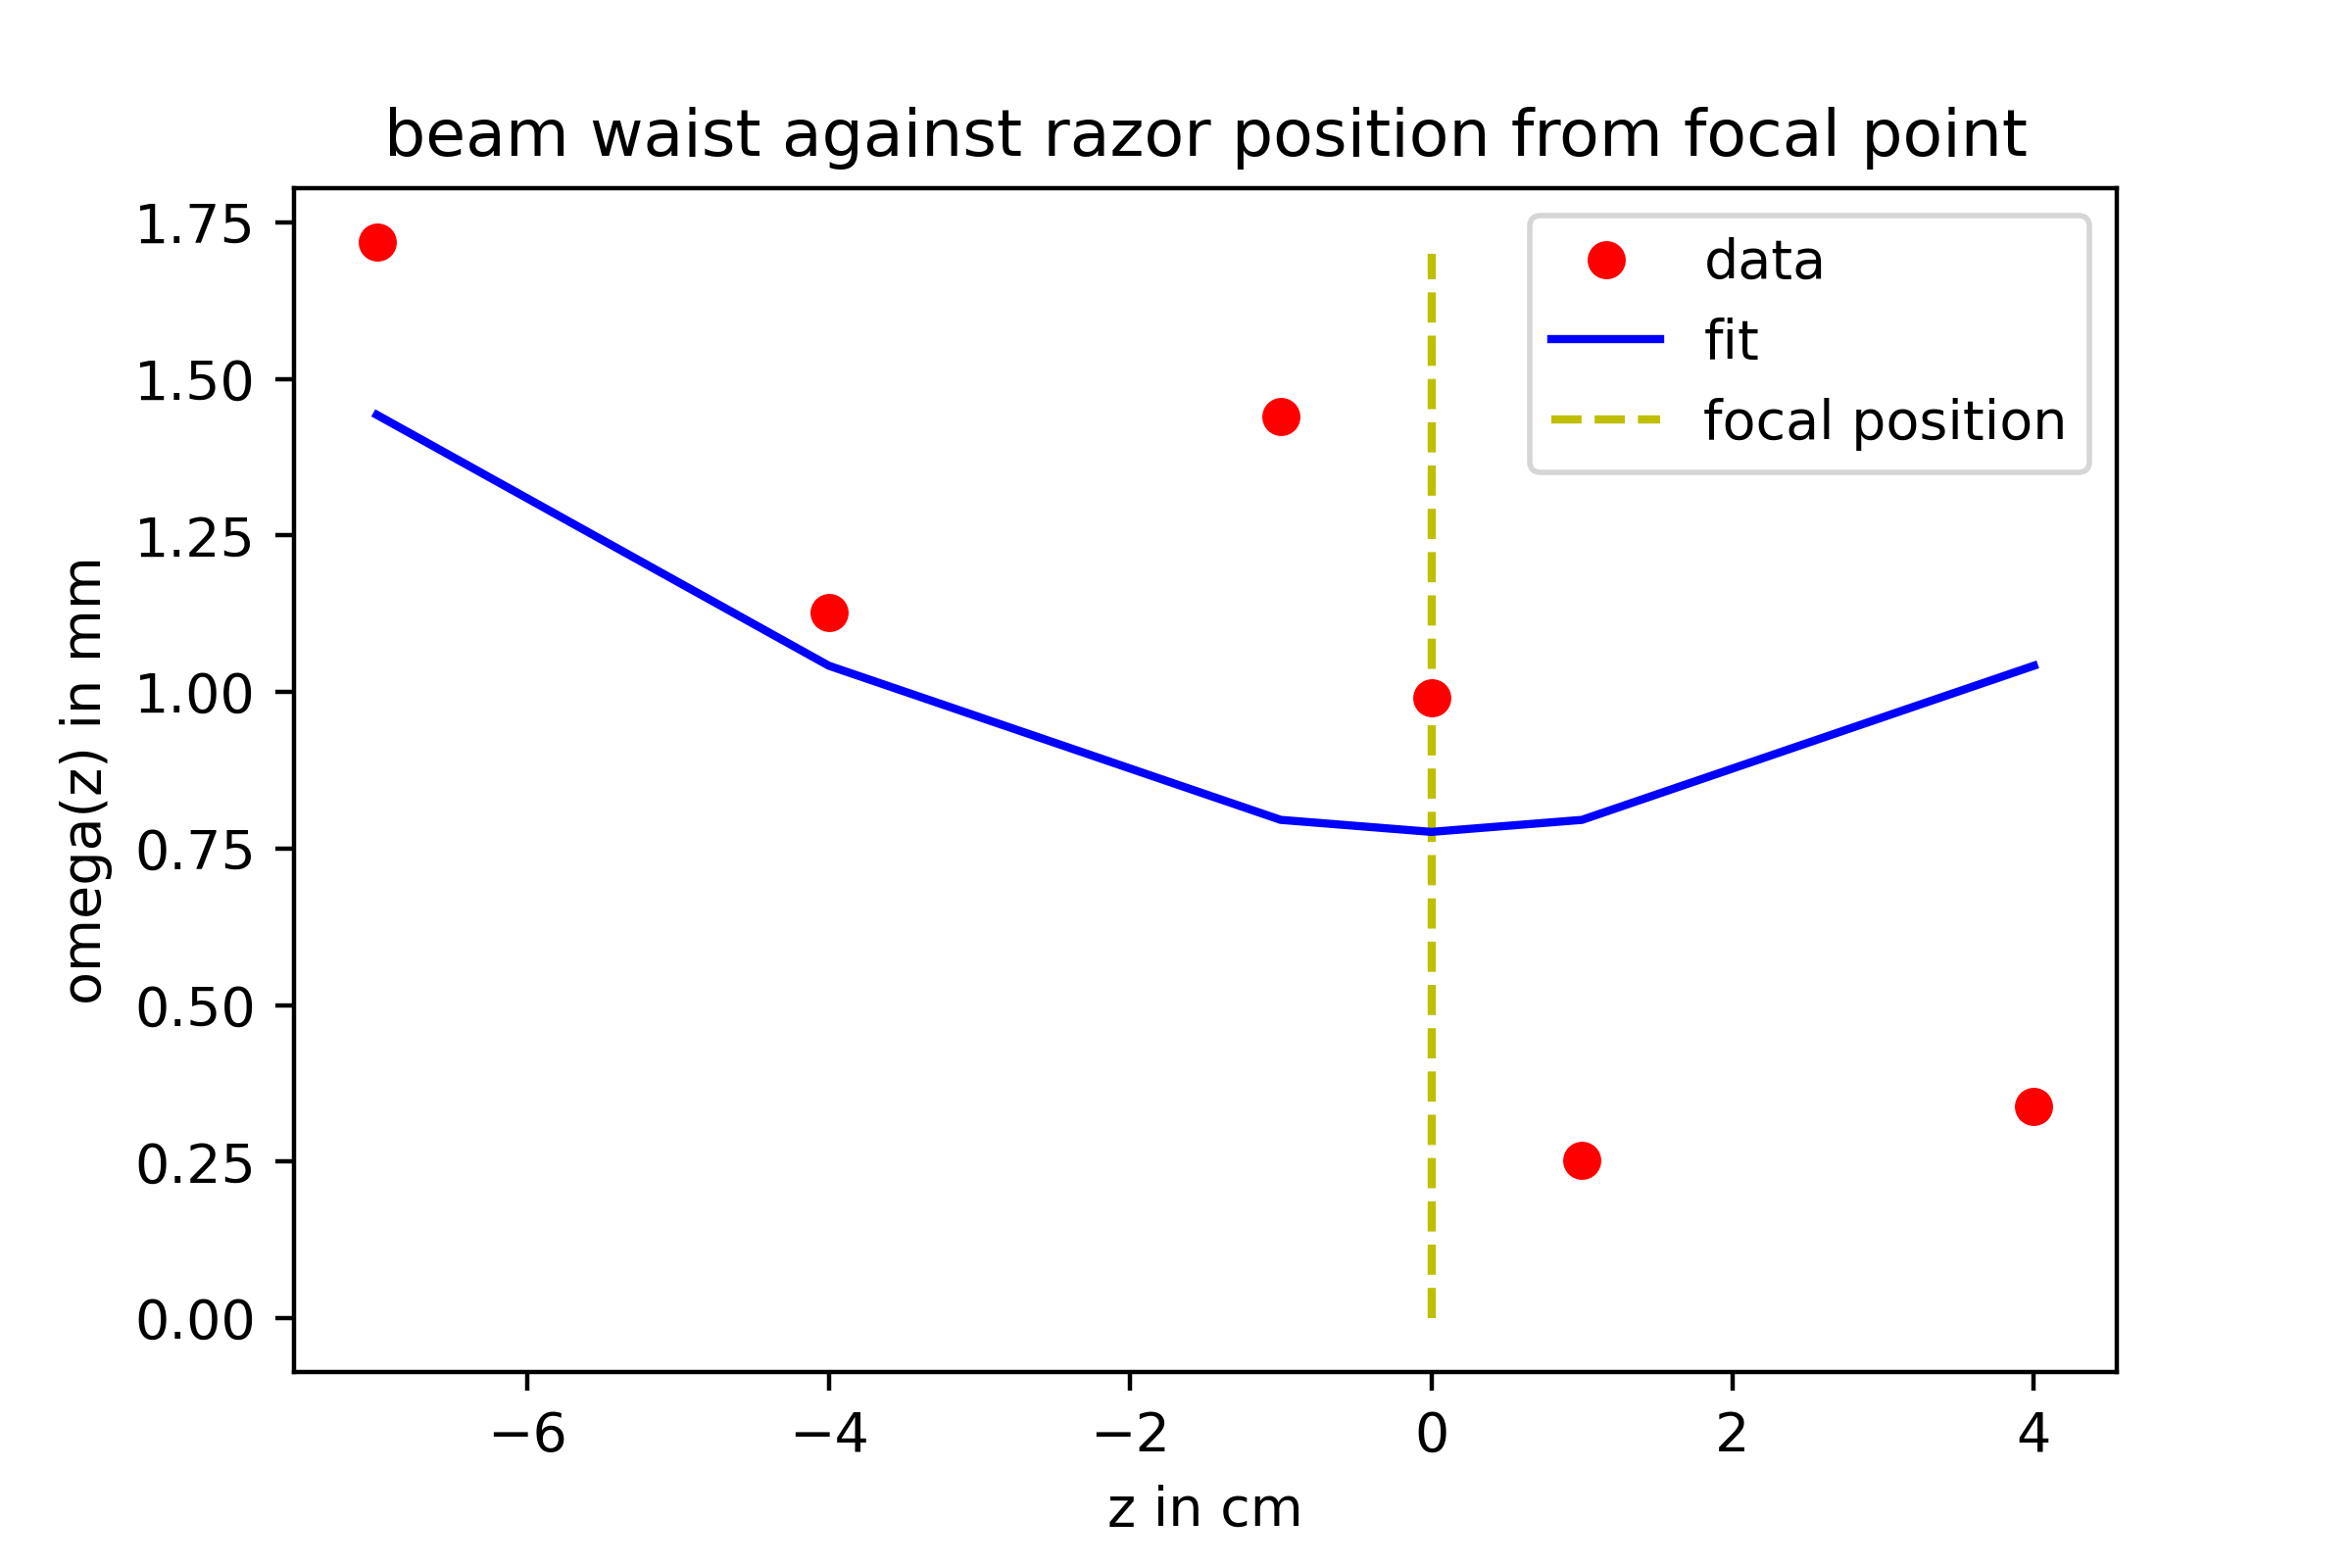
\includegraphics[width=\textwidth]{beam waist against razor position from focal point.png}

\textcolor{red}{
Wie müssen Sie eine plankonvexe Linse in diesem Fall orientieren, wenn Sie den Einfluß von Linsenfehlern möglichst gering halten wollen?}

\textcolor{red}{
Beschreibung Plot:
Messdaten:
Messungenauigkeiten Ursachen:
-At the focal point the multimeter display showed strong fluctuations}

\section{Optical resonator}

In the last part we constructed an optical resonator and detected the periodic signal of the beam that went through it with an oscilloscope. To do this we focused the beam on a lens 1 ($f=100mm$). Then we focused that on the movable reflector 1 with radius $r = 50mm$. In a distance $L=r$ (confocal arrangement) behind it we then positioned reflector 2 (same radius). The distance between lens 1 and reflector 1 is at first 50mm, so that the focal point of lens 1 lies exactly in the center of the optical resonator. At last we focused the beam into the center of a lens 2 and then into the photodiode with $R=100k\Omega$ (such that the signal is stronger), which we connected to the oscilloscope.

The measured signal looks like this:
\textcolor{red}{Bild einfügen, auch eine Skizze vom Versuchsaufbau}

\paragraph{Determining the transmission of the two reflectors}



\end{document}